
\chapter {Instructions for Installing and Setting Up Oscad}
The step by step instruction to install Oscad is given below.\\
Before starting the installation, first you need to meet system requirements and installation requirement. Installation script for Oscad is written in Bash.
This makes the installation efficient and user friendly. It is expected to have basic knowledge on Linux commands \\
\textbf{System Requirements:} \\
\begin{itemize}
\item Ubuntu 12.04 OS(64bit/32bit)
\item Oscad
\item Scilab 5.4.1
\end{itemize}
\textbf{Installation Requirements: }\\
\begin{itemize}
\item Working Internet connection
\item Require to be an admin user  to do the installation
\end{itemize}
\textbf{Prerequisites: }\\
\begin{itemize}
\item Basic knowledge of analog and digital electronics
\item Basic knowledge of Linux shell commands
\item Requires Synaptic Package Manager
\end{itemize}
%%%%%%%%%%%%%%%%%%%%%%%
\section {Procedure for installing Oscad}

\subsection {Step 1: Download Oscad and examples}
Go to \textbf{http://www.oscad.net/downloads}\\
Figure \ref{fig: Oscad Website} is shown below.\\
\newpage
\begin{figure}[h]
\centering
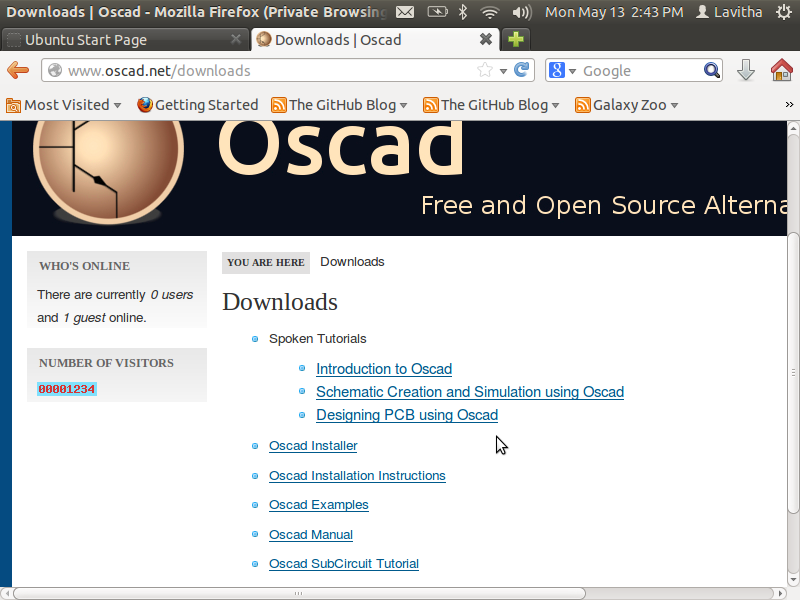
\includegraphics[width=0.9\textwidth]{figures/oscad1.png}
\caption{Oscad Website}
\label{fig: Oscad Website}
\end{figure}
\begin{itemize}
\item (a)Click on \textbf{Oscad Installer} and save the file in a folder\\
\item (b)Again click on \textbf{Oscad Examples} and save the file in same folder\\
\end{itemize}
%%%%%%%%%%%%%%%%%%%%%%%%%%%%
\subsection {Step 2: Check whether machine is 32bits or 64bits }
Go to Terminal and type\\
\Ovalbox{\textbf{uname -m} }\\and press enter\\
If the output is \textbf{i686}  then machine is 32 bits and if output is \textbf{x86\_64} then the machine is 64 bits.\\
Screen shot \ref{Terminall} shows that machine is 32 bits.
\begin{figure}[h!]
\centering
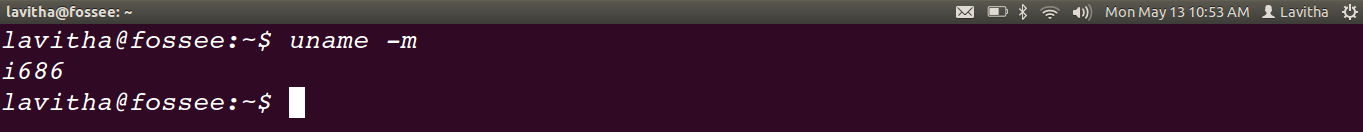
\includegraphics[width=0.9\textwidth]{figures/one.png}
\caption{Terminal}
\label{Terminall}
\end{figure}
%%%%%%%%%%%%%%%%%%%
\subsection {Step 3: Download Scilab }
Go to: \textbf{http://www.scilab.org/download/5.4.1} and download the scilab 5.4.1 under GNU/Linux section in the same folder where Oscad and \\
Examples were saved\\
Download scilab for 32 bits or 64 bits depending on the OS.\\
Figure \ref{scilab}  shows the options available under GNU/Linux
\begin{figure}[h!]
\centering
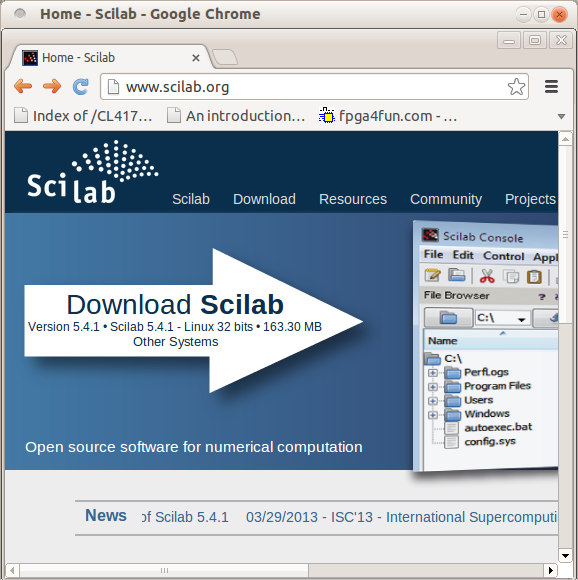
\includegraphics[width=0.9\textwidth]{figures/scilab.png}
\caption{scilab}
\label{scilab}
\end{figure}
%%%%%%%%%%%%%%%%%%%%%%%%%%
\subsection {Step 4: Extracting }
Go to folder where all the three folders are saved and do \textbf{extract here} 
%%%%%%%%%%%%%%%%%%%%%%%%%%%
\subsection {Step 5: Navigate to Folder  }
Go to folder where all the three folders are saved\\
For this go to terminal and type:\\
Note: Terminal commands are shown in box \\
\Ovalbox{\textbf{cd folder-where-downloaded-files-are-saved}} \\
Press Enter\\
Now check whether we have navigted to desired folder. To check please type:\\\\
\Ovalbox{\textbf{ls}}\\
Press Enter\\
Screen shot \ref{Terminalc} is shown below:
\begin{figure}[h!]
\centering
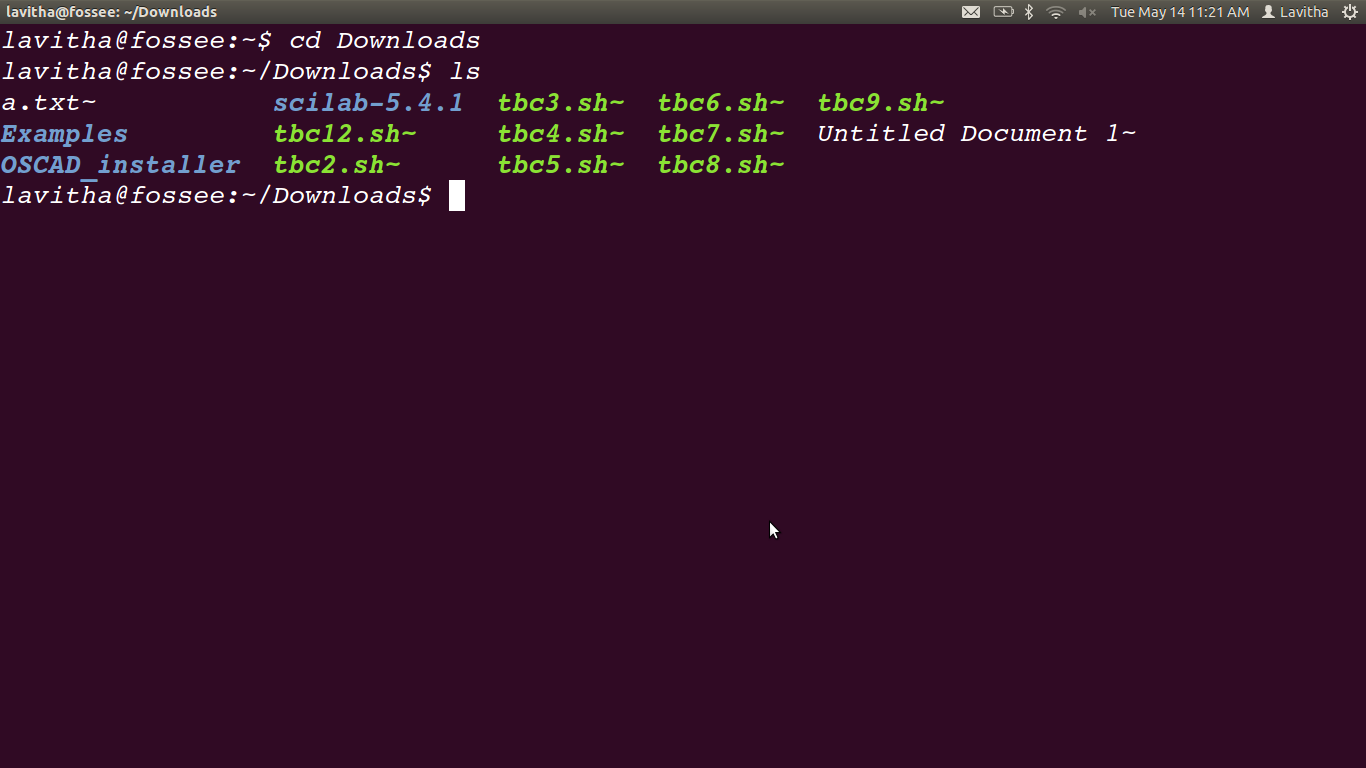
\includegraphics[width=0.9\textwidth]{figures/install0.png}
\caption{Terminal}
\label{Terminalc}
\end{figure}
%%%%%%%%%%%%%%%%%%%%%%%%%%%%%%
\subsection {Step 6: Navigate to OSCAD\_Installer}
Now navigate to OSCAD\_installer, To do this type:\\
\Ovalbox{\textbf{cd OSCAD\_installer}}\\
Press Enter
\begin{figure}[h!]
\centering
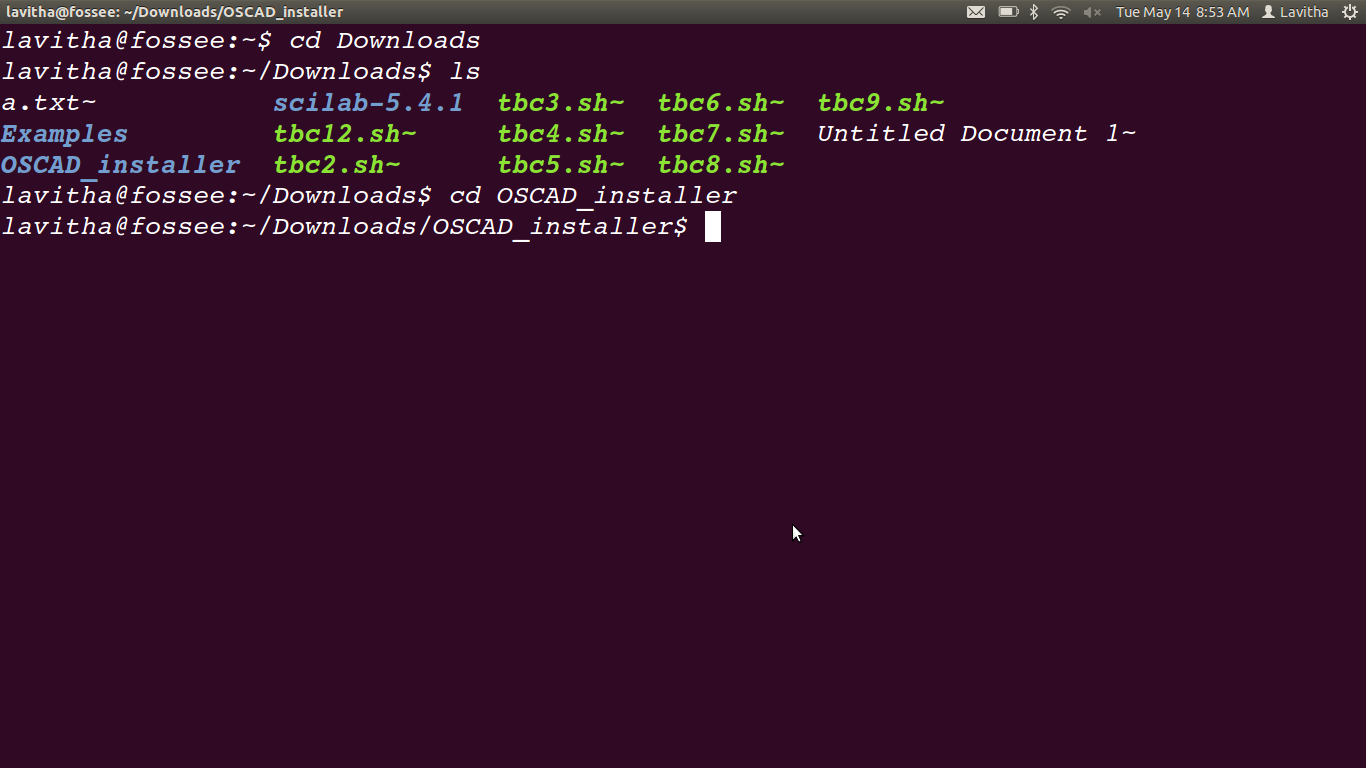
\includegraphics[width=0.9\textwidth]{figures/installer1.png}
\caption{Terminal}
\label{Terminal}
\end{figure}
%installer1.png

%%%%%%%%%%%%%%%%%%%%%%%%%%%%%%%%%%%%%
\subsection {Step 7: Make the installOSCAD and \\
installModule files executable }
To do this go to terminal and Type:\\
\Ovalbox{\textbf{sudo chmod 755 installOSCAD.sh installModule.sh}}\\
Press Enter\\
Type the sudo(root) password\\
The Terminal should look like below as shown in figure \ref{term}
\newpage
\begin{figure}[h!]
\centering
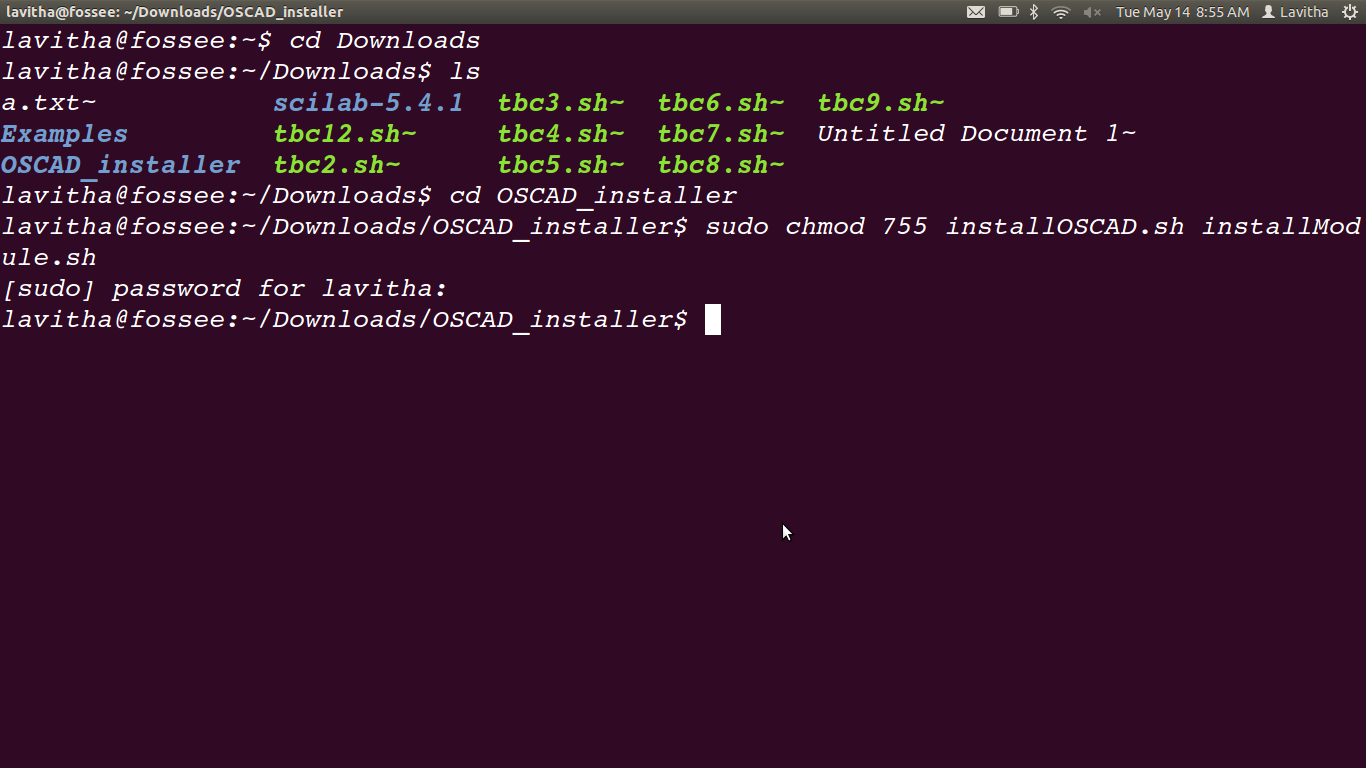
\includegraphics[width=0.9\textwidth]{figures/install3.png}
\caption{Terminal: To make executable}
\label{term}
\end{figure}
%%%%%%%%%%%%%%%%%%%%%%%%%%%%%%%%%%%%%%%%%%%%%
\subsection {Step 8: Begin installation }
To begin installation, on the Terminal type\\
\Ovalbox{\textbf{ ./installOscad.sh}}\\
Press Enter\\
The Terminal prompts for proxy setting as shown in \ref{proxy}
\begin{figure}[h!]
\centering
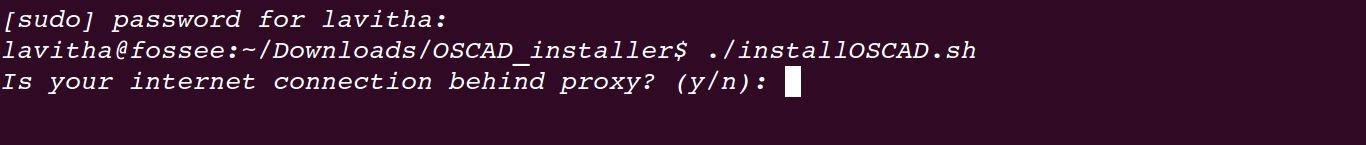
\includegraphics[width=0.9\textwidth]{figures/install4.png}
\caption{Terminal: Installation}
\label{proxy}
\end{figure}\\
Enter the related proxy details as shown in figure \ref{proxys}
\begin{figure}[h]
\centering
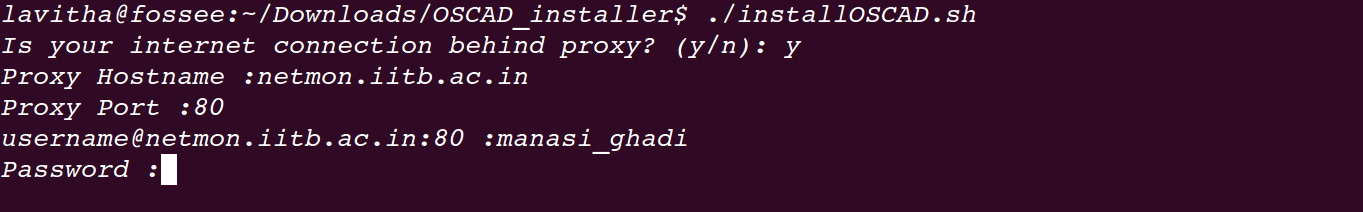
\includegraphics[width=0.9\textwidth]{figures/install5.png}
\caption{Terminal: Proxy}
\label{proxys}
\end{figure}
\newline
Now the prompt displays message 
\textbf{Do you want to continue [Y/n]:}\\
Type 'y' and press Enter. Kicad, ngspice and necessary python modules will be installed.\\
Note: While installing the python modules, you may get some error messages.
In that case, install the missing packages using Synaptic Package Manager. 
Once this is done, re-run the installOscad.sh script.
%%%%%%%%%%%%%%%%%%%%%%%%%%%%%%%%%%%%%%
\subsection {Step 9: Linking of Scilab}
The prompt displays the message:\\
\textbf{Do you have scilab5.4 or above? (y/n)}\\
\begin{figure}[h]
\centering
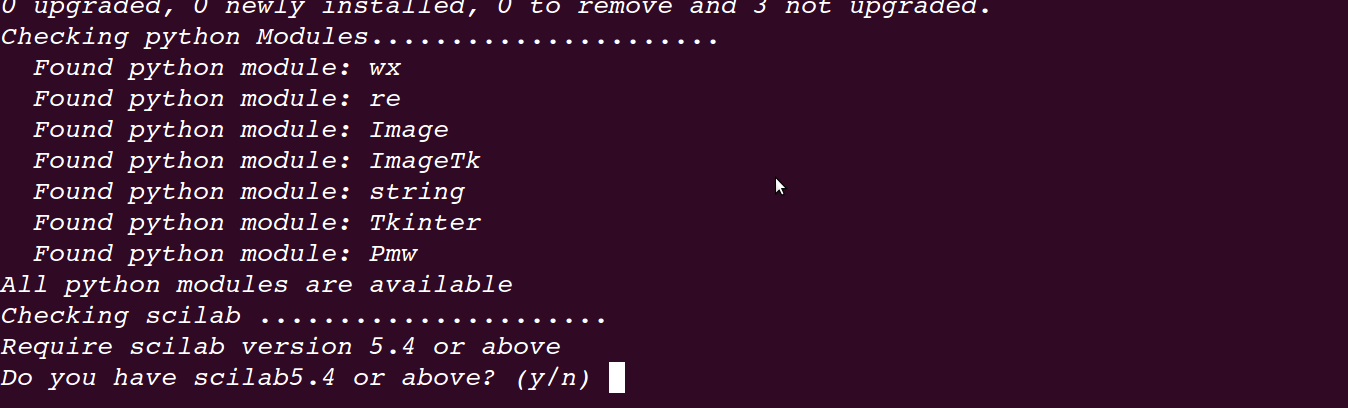
\includegraphics[width=0.9\textwidth]{figures/install6.png}
\caption{Terminal: To make executable}
\label{Terminal: make executable}
\end{figure}
\newpage
Type: 'y' and press Enter\\
Now give the complete path:
on Terminal:\\
Example:
\textbf{\Ovalbox{/home/lavitha/downloads/scilab-5.4.1}}\\
The screen shot is shown below:\\
\begin{figure}[h]
\centering
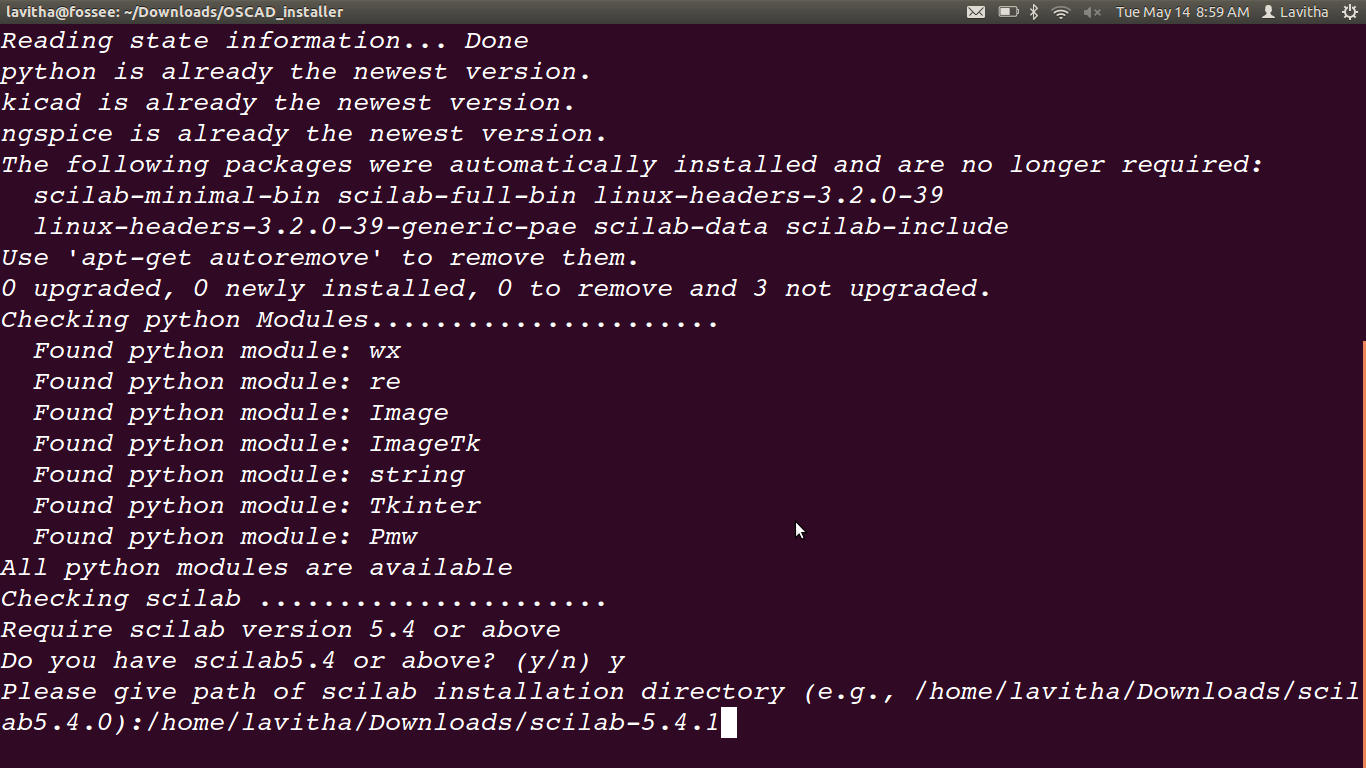
\includegraphics[width=0.9\textwidth]{figures/install7.png}
\caption{Terminal: Scilab instllation}
\label{Terminal: make executable}
\end{figure}
and Press enter\\
The \textbf{metanet toolbox} is installed and this take couple of minutes\\
%%%%%%%%%%%%%%%%%%%%%%%
\subsection {Step 10: Final installation}
The prompt displays the message

\Ovalbox{\textbf{Please select installation directory}}\\
Select the desired location and press Enter\\
For example:\\
\Ovalbox{\textbf{/home/lavitha}}\\
Press Enter\\
If everything is installed then prompt displays message\\
\textbf{installation completed}\\
\begin{figure}[h]
\centering
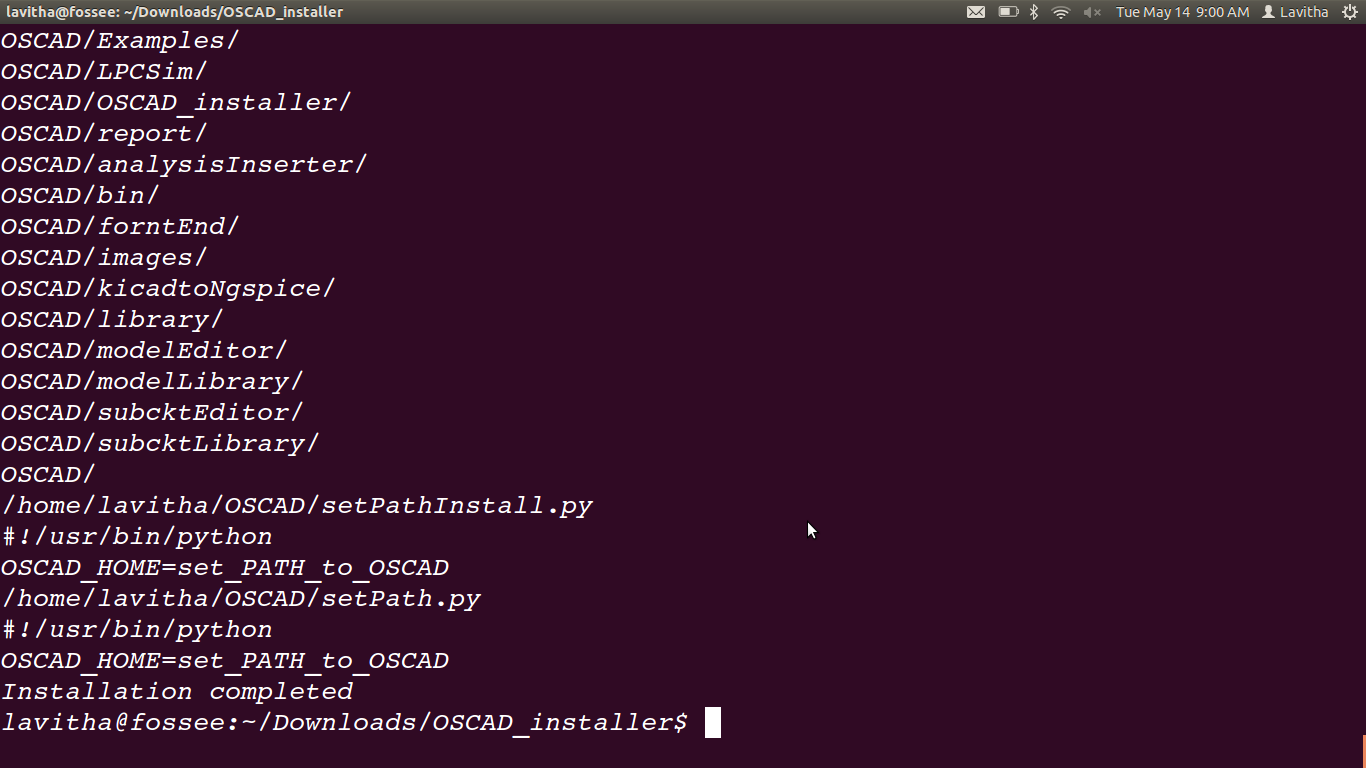
\includegraphics[width=0.9\textwidth]{figures/install9.png}
\caption{Terminal: Installation Completed}
\label{Terminal: Installation completed}
\end{figure}
This creates textbf{Oscad} shortcut on Desktop.
%%%%%%%%%%%%%%%%%%%%%%%%
\subsection {Step 11: Testing}
\begin{itemize}
\item Double click on Oscad shortcut created on Desktop as shown below:
\begin{figure}[h]
\centering
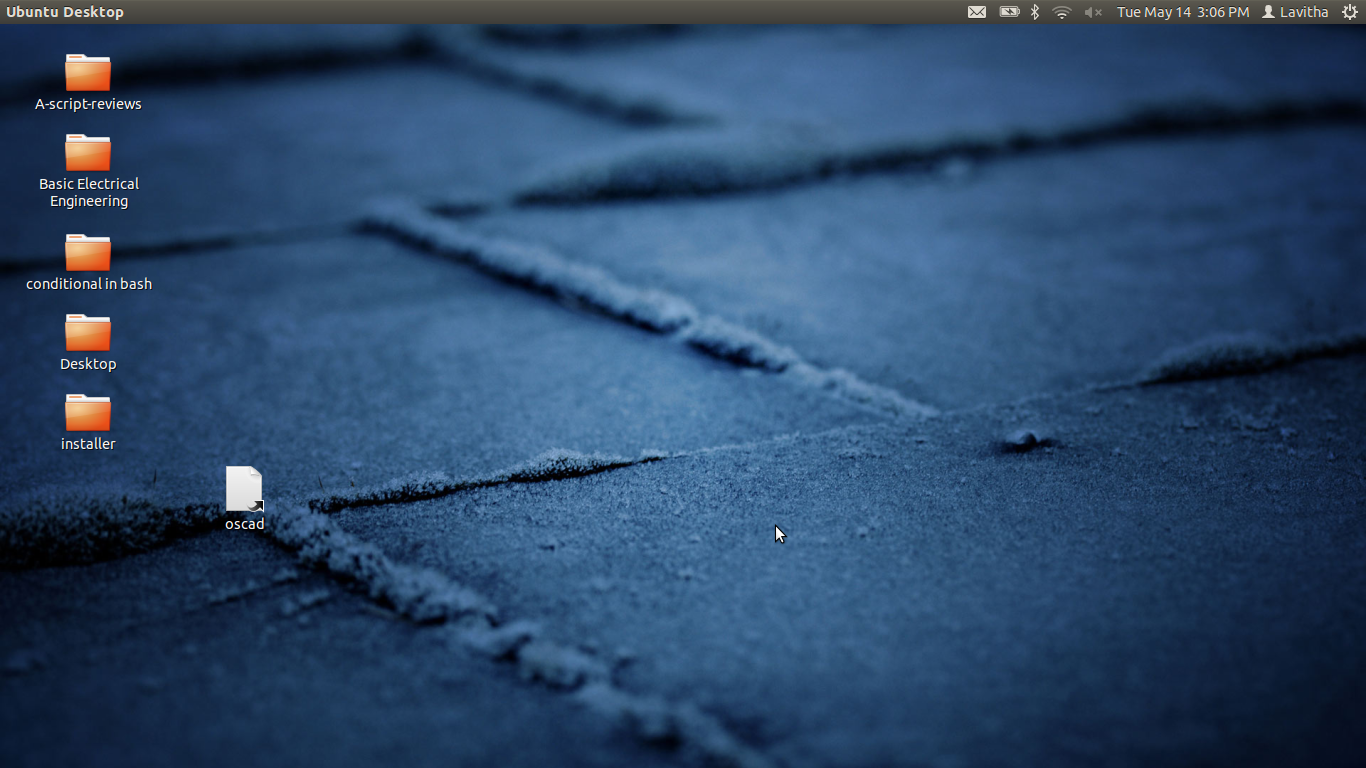
\includegraphics[width=0.9\textwidth]{figures/screenshot1.png}
\caption{Desktop: Oscad shortcut}
\label{Terminal: Oscad shortcut}
\end{figure}
\newpage
\item A tab is displayed as shown below. select \textbf{Run option}
\begin{figure}[h]
\centering
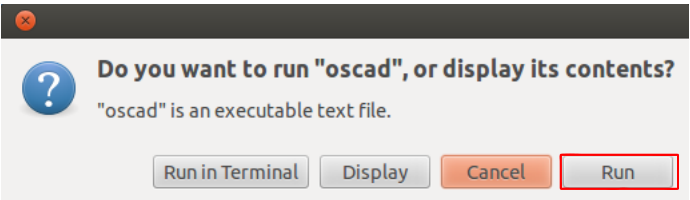
\includegraphics[width=0.9\textwidth]{figures/run.png}
\caption{Desktop: Oscad }
\label{Terminal: Oscad}
\end{figure}
\item It opens the Oscad window as show below:
\begin{figure}[h]
\centering
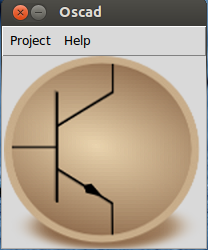
\includegraphics[width=0.6\textwidth]{figures/oscadicon.png}
\caption{Desktop: Oscad }
\label{Terminal: Oscad}
\end{figure}
\newpage
\item select \textbf{project} and then \textbf{open}
Browse the folder where examples is saved
\item Double click on Examples
\item select \textbf{RC} from the examples by double clicking on RC

\end{itemize}




